\documentclass[12pt]{article}

\usepackage[pdftex]{graphicx}
\usepackage{amsmath}
\usepackage{enumitem}


\newcommand\tab[1][1cm]{\hspace*{#1}}
\newcommand{\HRule}{\rule{\linewidth}{0.5mm}}

% Margins
\topmargin=-0.45in
\evensidemargin=0in
\oddsidemargin=0in
\textwidth=6.5in
\textheight=9.0in
\headsep=0.25in
\title{ COMS 474\\Homework 3 }
\author{ Haadi Majeed }
\date{Spring 2022}

\usepackage{cancel}
\usepackage[margin=4cm]{geometry}
\usepackage[hidelinks]{hyperref}
\usepackage{fancyhdr}
\pagestyle{fancy}
\fancyhead{}
\fancyfoot{}
\lhead{COMS 474}
\chead{Haadi Majeed}
\rhead{Page \thepage}

\begin{document}
\maketitle
\pagebreak

% Optional TOC
% \tableofcontents
% \pagebreak
\section*{Problem 1}
 [26 points total ]\\
For the following, you will look at how the underlying $f(X)$ and the number of samples play a role in the occurrence and extent of both under-fitting and over-fitting. You will use the Jupyter notebook posted on canvas along with these directions. You should only need to modify two variables in the last code block, setting $f\_type$ to ‘linear’ or ‘sinusoidal’ and setting $n\_samples$ to 15 or 1000.
\\\\
Recall that there are many factors that affect how well a fitted model will perform on future data, including the class of models we are using for fitting (here polynomials), the underlying trend $f(X)$, the noise (here additive Gaussian), and the number of samples.
\\\\
\textbf{\underline{Additional Notes}}
\begin{itemize}
    \item The results are random, since the data set itself is random.
    \item You are encouraged to re-run the code for each setting a few times to gain some insight into the variability of the results. We will explore this issue in more depth later on.
    \item The $Y$ axis for the MSE figure does not have fixed limits. Pay attention to the range of the MSE values as you compare plots.
\end{itemize}

\begin{enumerate}[label=(\alph*)]
    \item Using a sinusoidal $f(X)$ and noise standard deviation $\sigma = 5$, plot the estimated models and the MSE curves for
          \begin{enumerate}[label=(\roman*)]
              \item $n = 15$ samples
              \item $ n = 1000$ samples
          \end{enumerate}
          Using those four plots, comment on whether under-fitting and/or over-fitting occur and the extent to which they do for each of i. and ii. Then discuss how the number of samples affects the result (eg similarities and differences between i. and ii.)\\
          \begin{center}
              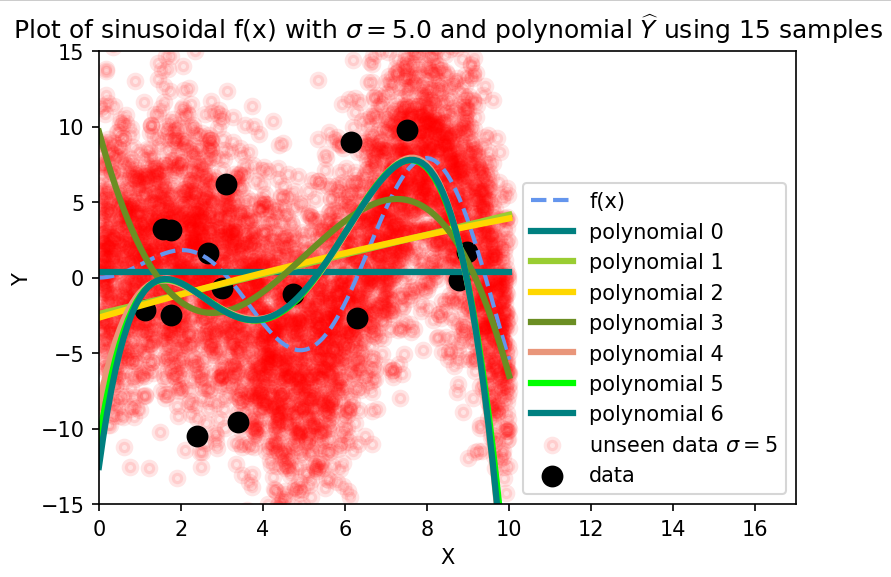
\includegraphics[width=1\textwidth]{sinosodial-15.png}
              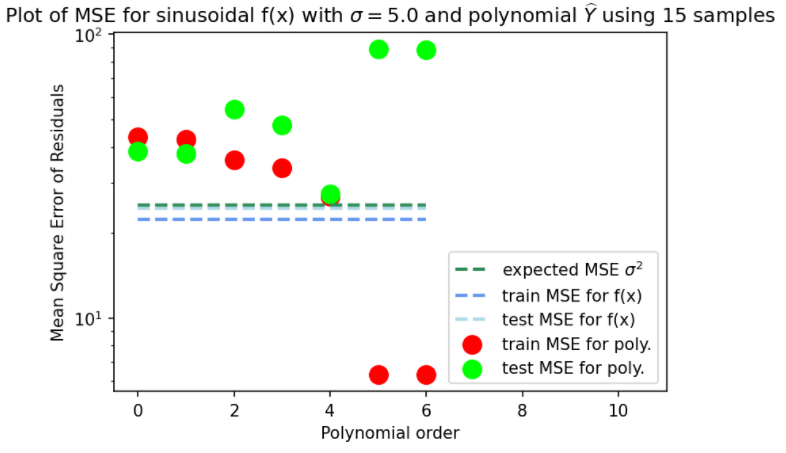
\includegraphics[width=1\textwidth]{sinosodial-MSE-15.png}
              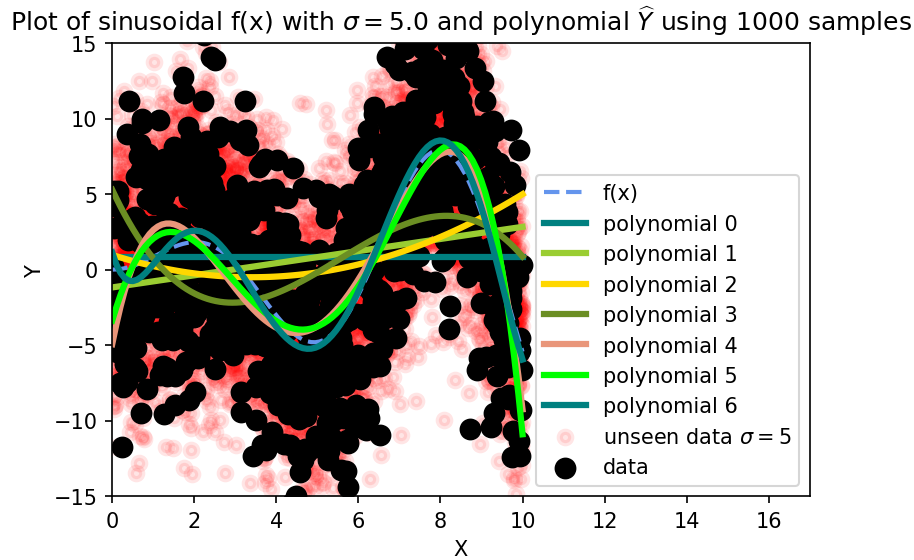
\includegraphics[width=1\textwidth]{sinosodial-1000.png}
              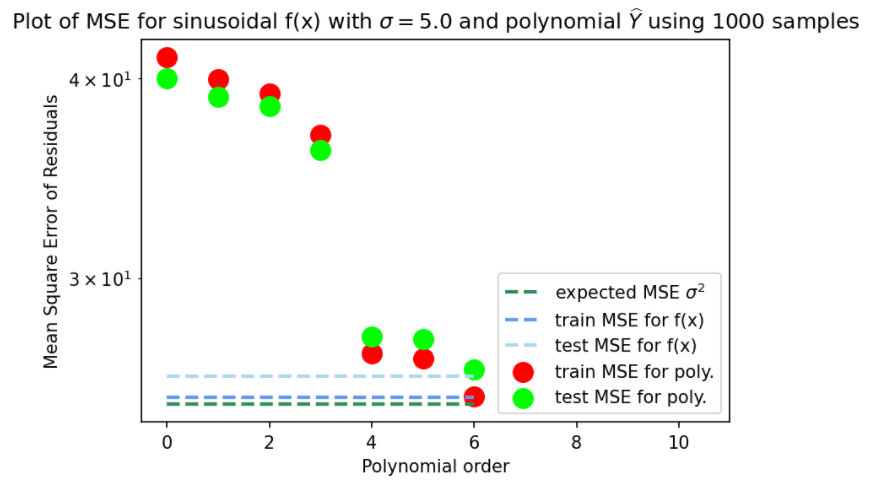
\includegraphics[width=1\textwidth]{sinosodial-MSE-1000.png}
          \end{center}
          \begin{enumerate}[label=(\roman*)]
              \item When looking at the model of sinosodial with 15 samples, a few things can be noticed, in the instance that I have attached, polynomial models 5 and 6 are great instances of overfitting the data and can be deemed as such as they hit or get very close almost every test data point in the set of 15 available for it to hit, while polynomial models 0 and 1 are showing processing that there is a signifigant amount of error in the system and underfits the data by linearly cutting through it all, almost averaging it out for model 1.
              \item When looking at the sinusoidal with 1000 samples, determining how something fits becomes more difficult, visually at least, it can be said that polynomial models 0 and 1 once again severely underfit the data as ignore many attributes of the data, labeling it as error. However, the higher polynomial models like 4 and 5, but more importantly 6, it is harder to determine if they are overfitting or not due to the sheer number of data points it contains, however to truly overfit, the flexibility would need to be unreasonably high.
          \end{enumerate}
          \pagebreak
    \item Repeat (a) with a linear $f(X)$.
          \begin{center}
              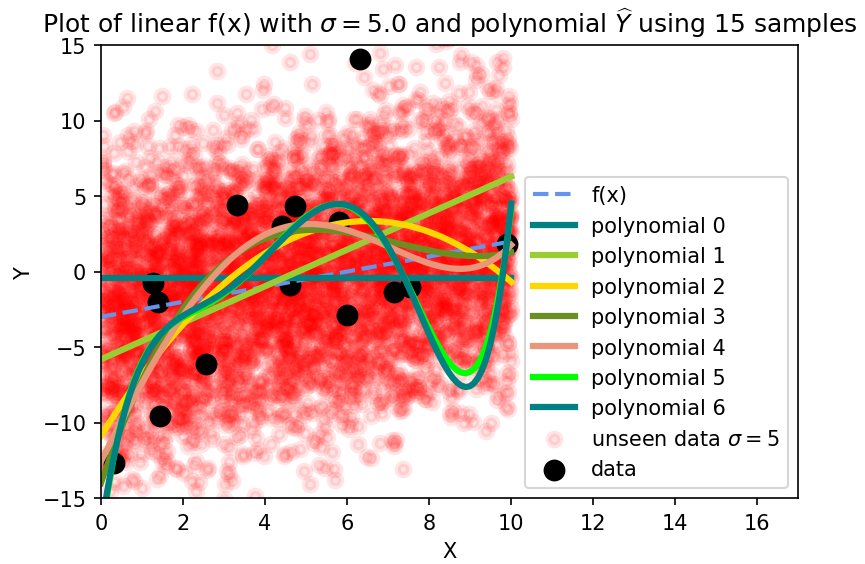
\includegraphics[width=1\textwidth]{linear-15.png}
              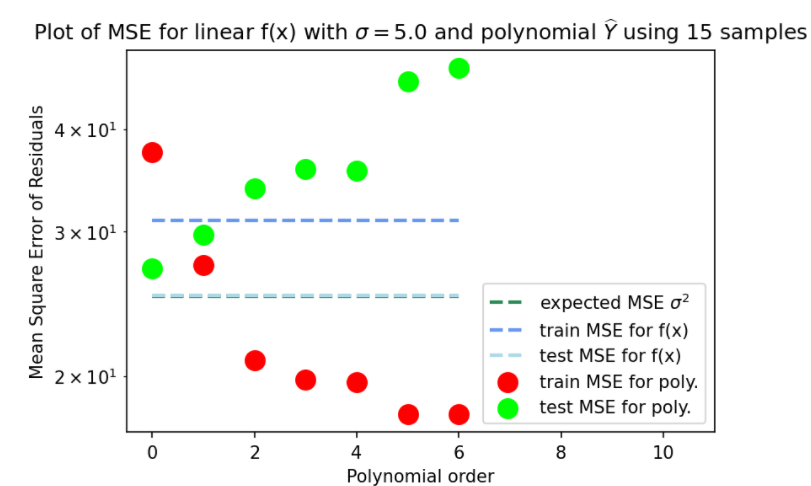
\includegraphics[width=1\textwidth]{linear-MSE-15.png}
              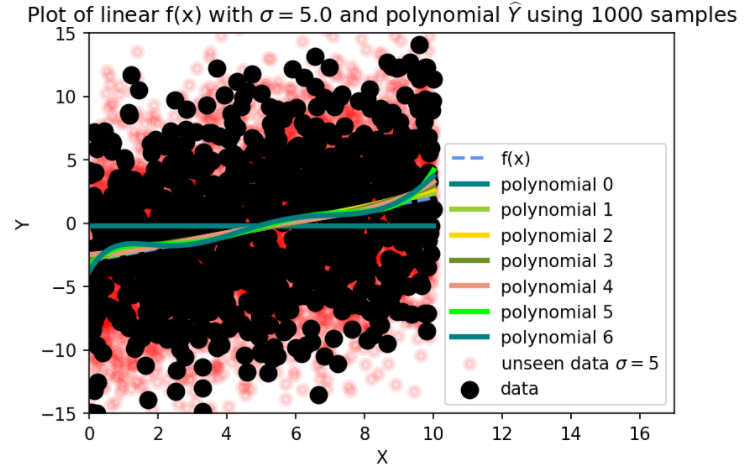
\includegraphics[width=1\textwidth]{linear-1000.png}
              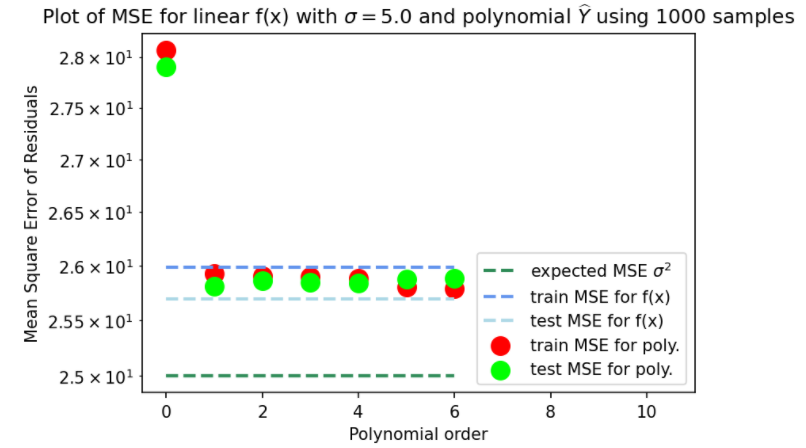
\includegraphics[width=1\textwidth]{linear-MSE-1000.png}
          \end{center}
          \begin{enumerate}[label=(\roman*)]
              \item When looking at the linear model with 15 samples, the models that have a polynomial try to fit all the data, ignoring much of the variance and taking them as true data points which when compared to the true model, we know is not what it should be doing. However the models that are lower in polynomial fit the data better, especially the first order model, as it is quite close.
              \item The linear model with 1000 samples is a bit more difficult to interpret, however one thing we can notice immeditely is that most models look fairly linear and lean the same way as the base model. We again encounter the issue that overfitting this much data would be harder, but as is, all models above base 0 closely match each other and all fall within the margins set by the training MSE and testing MSE which is quite impresive when compared to the previous 3 models.
          \end{enumerate}
    \item Now discuss similarities and differences between the results of (a) and (b), given that the main difference was $f(X)$ (which for (a) was not only non-linear in $X$ but also not in the model class we were fitting with, while for (b) it was linear and in the model class).\\

\end{enumerate}
%--/Paper--

\end{document}